% Copyright 2004 by Till Tantau <tantau@users.sourceforge.net>.
%
% In principle, this file can be redistributed and/or modified under
% the terms of the GNU Public License, version 2.
%
% However, this file is supposed to be a template to be modified
% for your own needs. For this reason, if you use this file as a
% template and not specifically distribute it as part of a another
% package/program, I grant the extra permission to freely copy and
% modify this file as you see fit and even to delete this copyright
% notice. 

\documentclass{beamer}
% Replace the \documentclass declaration above
% with the following two lines to typeset your 
% lecture notes as a handout:
%\documentclass{article}
\usepackage{CJKutf8}
\usepackage[T1]{fontenc}
%\usepackage[utf8x]{inputenc}
\usepackage{graphicx}
\usepackage{ulem}
\usepackage{url}

% There are many different themes available for Beamer. A comprehensive
% list with examples is given here:
% http://deic.uab.es/~iblanes/beamer_gallery/index_by_theme.html
% You can uncomment the themes below if you would like to use a different
% one:
%\usetheme{AnnArbor}
%\usetheme{Antibes}
%\usetheme{Bergen}
%\usetheme{Berkeley}
%\usetheme{Berlin}
%\usetheme{Boadilla}
%\usetheme{boxes}
%\usetheme{CambridgeUS}
%\usetheme{Copenhagen}
%\usetheme{Darmstadt}
%\usetheme{default}
%\usetheme{Frankfurt}
\usetheme{Goettingen}
%\usetheme{Hannover}
%\usetheme{Ilmenau}
%\usetheme{JuanLesPins}
%\usetheme{Luebeck}
%\usetheme{Madrid}
%\usetheme{Malmoe}
%\usetheme{Marburg}
%\usetheme{Montpellier}
%\usetheme{PaloAlto}
%\usetheme{Pittsburgh}
%\usetheme{Rochester}
%\usetheme{Singapore}
%\usetheme{Szeged}
%\usetheme{Warsaw}

\begin{document}
\begin{CJK}{UTF8}{gbsn}

\title{Cassandra分布式NoSQL存储简介}

% A subtitle is optional and this may be deleted
\subtitle{原理与应用}

\author{李庚\inst{1}}
% - Give the names in the same order as the appear in the paper.
% - Use the \inst{?} command only if the authors have different
%   affiliation.

\institute[Qunar.com] % (optional, but mostly needed)
{
  \inst{1}%
  旅游度假事业部
  Qunar.com
}
% - Use the \inst command only if there are several affiliations.
% - Keep it simple, no one is interested in your street address.

\date{Mar. 5th, 2015}
% - Either use conference name or its abbreviation.
% - Not really informative to the audience, more for people (including
%   yourself) who are reading the slides online

\subject{2015度假部门技术分享}
% This is only inserted into the PDF information catalog. Can be left
% out. 

% If you have a file called "university-logo-filename.xxx", where xxx
% is a graphic format that can be processed by latex or pdflatex,
% resp., then you can add a logo as follows:

% \pgfdeclareimage[height=0.5cm]{university-logo}{university-logo-filename}
% \logo{\pgfuseimage{university-logo}}

% Delete this, if you do not want the table of contents to pop up at
% the beginning of each subsection:
\AtBeginSubsection[]
{
  \begin{frame}<beamer>{纲要}
    \tableofcontents[currentsection,currentsubsection]
  \end{frame}
}

% Let's get started

\begin{frame}
  \titlepage
\end{frame}

\begin{frame}{纲要}
  \tableofcontents
  % You might wish to add the option [pausesections]
\end{frame}

% Section and subsections will appear in the presentation overview
% and table of contents.
\section{Cassandra是什么}

\subsection{概览}
\begin{frame}{懒人使用手册}
  \begin{itemize}
  \item {
      CREATE KEYSPACE my\_test\_ks WITH replication = \{'class': 'SimpleStrategy', 'replication\_factor': 3\};

      \pause
  }
  \item {
      USE my\_test\_ks;

      \pause
  }
  \item {
      CREATE TABLE my\_table(key1 text, key2 int, value1 text, value2 int, PRIMARY KEY (key1, key2));

      \pause
  }
  \item {
      INSERT INTO my\_table (key1, key2, value1, value2) VALUES ('kk', 33, 'vv', 66);
      UPDATE my\_table SET value1 = 'vvv' WHERE key1 = 'kk' and key2 = 33;

      \pause
  }
  \item {
      SELECT * FROM my\_table WHERE key1 = 'kk' and key2 = 33;
  }
  \end{itemize}
\end{frame}

\subsection{特性描述}
\begin{frame}{主要特点}
  \begin{itemize}
  \item {
      分布式Key-Value型数据存储
  }
  \pause
  \item {
      Horizontal Scaling: 数据量级膨胀时,可通过加服务器节点的方式解决。
  }
  \pause
  \item {
      无中心节点的概念(P2P),无单点瓶颈
  }

  \pause
  \item {
      自动机群维护
  }
  \end{itemize}
\end{frame}

\section{技术实现原理}

\begin{frame}{两篇文章}
  \begin{block}{Dynamo: Amazon’s Highly Available Key-value Store, SOSP 2007}
    \begin{itemize}
    \item {一致性哈希(Consistent hashing)}
    \item {数据副本分布}  
    \end{itemize}
  \end{block}
  \begin{block}{BigTable: A Distributed Structured Storage System, OSDI 2006}
    \begin{itemize}
    \item {SSTable, Memtable数据结构}
    \item {Column Family的概念}
    \end{itemize}
  \end{block}
\end{frame}

\subsection{数据如何分布在不同的服务节点上?}

\begin{frame}{可配置副本个数的存储}
  \begin{itemize}
  \item {
      复制因子(Replication Factor): 每个主键对应的数据项有多少个副本
  }
  \item {
      一致性级别(Consistency Level): 读/写操作在多少个副本上返回才认为这次操作是成功的(依据业务需要进行取舍)
  }
  \end{itemize}
  \pause
  \begin{block}{将Key通过一致性哈希运算映射到环状拓扑结构中的某些节点上}
  \begin{center}
    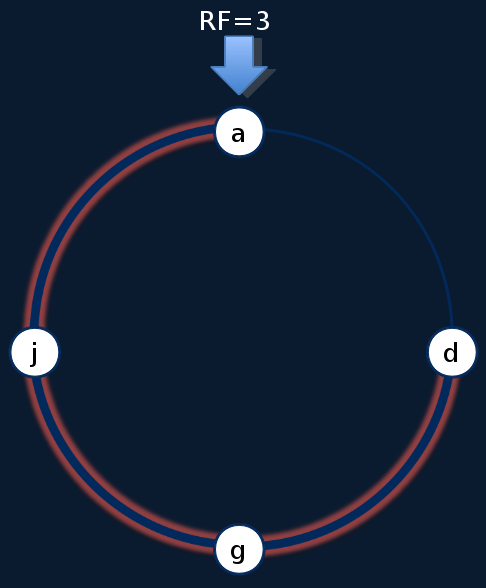
\includegraphics[scale=0.22]{./images/ring-topology-rf3}
  \end{center}
  \end{block}
\end{frame}

\begin{frame}{新增节点}
  \begin{center}
    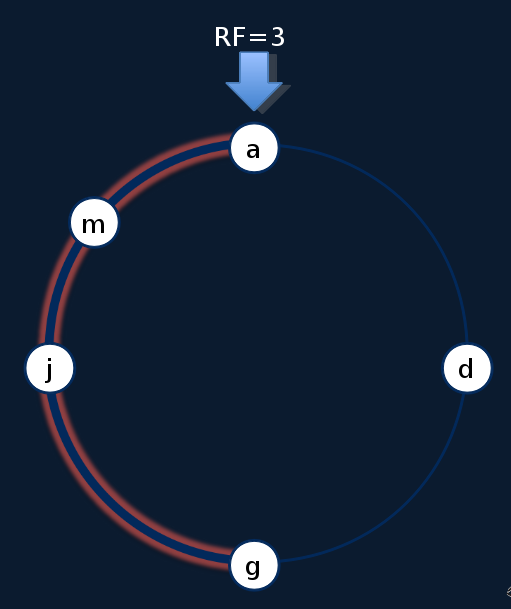
\includegraphics[scale=0.22]{./images/new-node}
  \end{center}
\end{frame}

\subsection{存储结构模型}
\begin{frame}{列}
  \begin{center}
    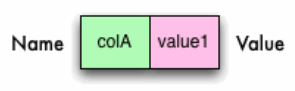
\includegraphics[scale=0.4]{./images/column}
  \end{center}
\end{frame}

\begin{frame}{行}
  \begin{center}
    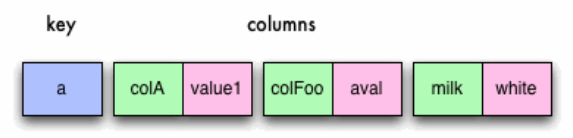
\includegraphics[scale=0.4]{./images/row}
  \end{center}
\end{frame}

\begin{frame}{表}
  \begin{center}
    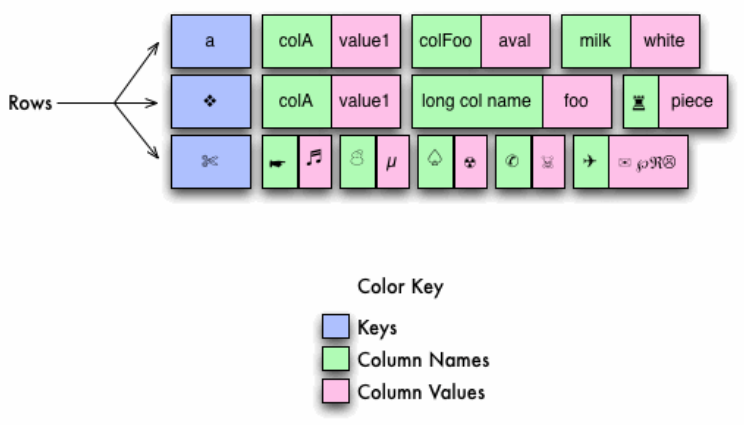
\includegraphics[scale=0.3]{./images/table}
  \end{center}
\end{frame}


\subsection{单节点上的读、写过程}

\begin{frame}{写入:性能极好}
  \begin{center}
    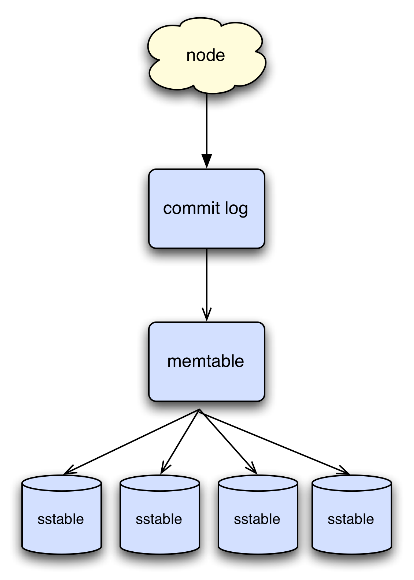
\includegraphics[scale=0.4]{./images/write-process}
  \end{center}
\end{frame}

\begin{frame}{}
  \begin{block}{Commit Log: 保证持久性}
    \begin{itemize}
    \item {只能顺序追加}
    \end{itemize}
  \end{block}
  \pause
  \begin{block}{Memtable数据结构}
    \begin{itemize}
    \item {不需磁盘访问}
    \end{itemize}
  \end{block}
  \pause
  \begin{block}{SSTable外存数据结构: 只读}
    \begin{itemize}
    \item {索引}
    \item {Bloom Filter}
    \item {数据副本}
    \end{itemize}
  \end{block}
\end{frame}

\begin{frame}{读取:基本上不会被阻塞}
  \begin{center}
    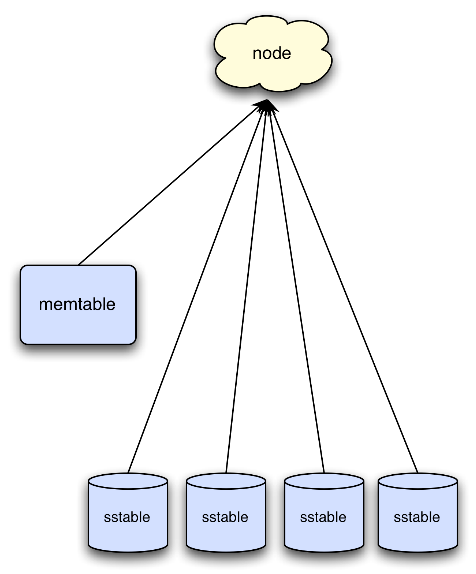
\includegraphics[scale=0.4]{./images/read-process}
  \end{center}
\end{frame}

\begin{frame}{}
  \begin{block}{必须指定Key(主键或者Partition Key)}
    \begin{itemize}
      \item {单一:key = 'a'}
      \item {区间: key = 'a' through 'f'}
    \end{itemize}
  \end{block}
  \pause
  \begin{block}{不能像SQL那样用where clause对任意属性查询}
    \begin{itemize}
      \item {需要分布到多个节点进行全表扫描,代价太高}
      \item {若有需要的话,可通过运行Spark, Hadoop程序实现}
    \end{itemize}
  \end{block}
\end{frame}


\section{使用经验}

\subsection{应用范围}

\begin{frame}{部署规模}
  \begin{block}{复用度假搜索倒排索引服务器,跨机房部署}
    \begin{center}
      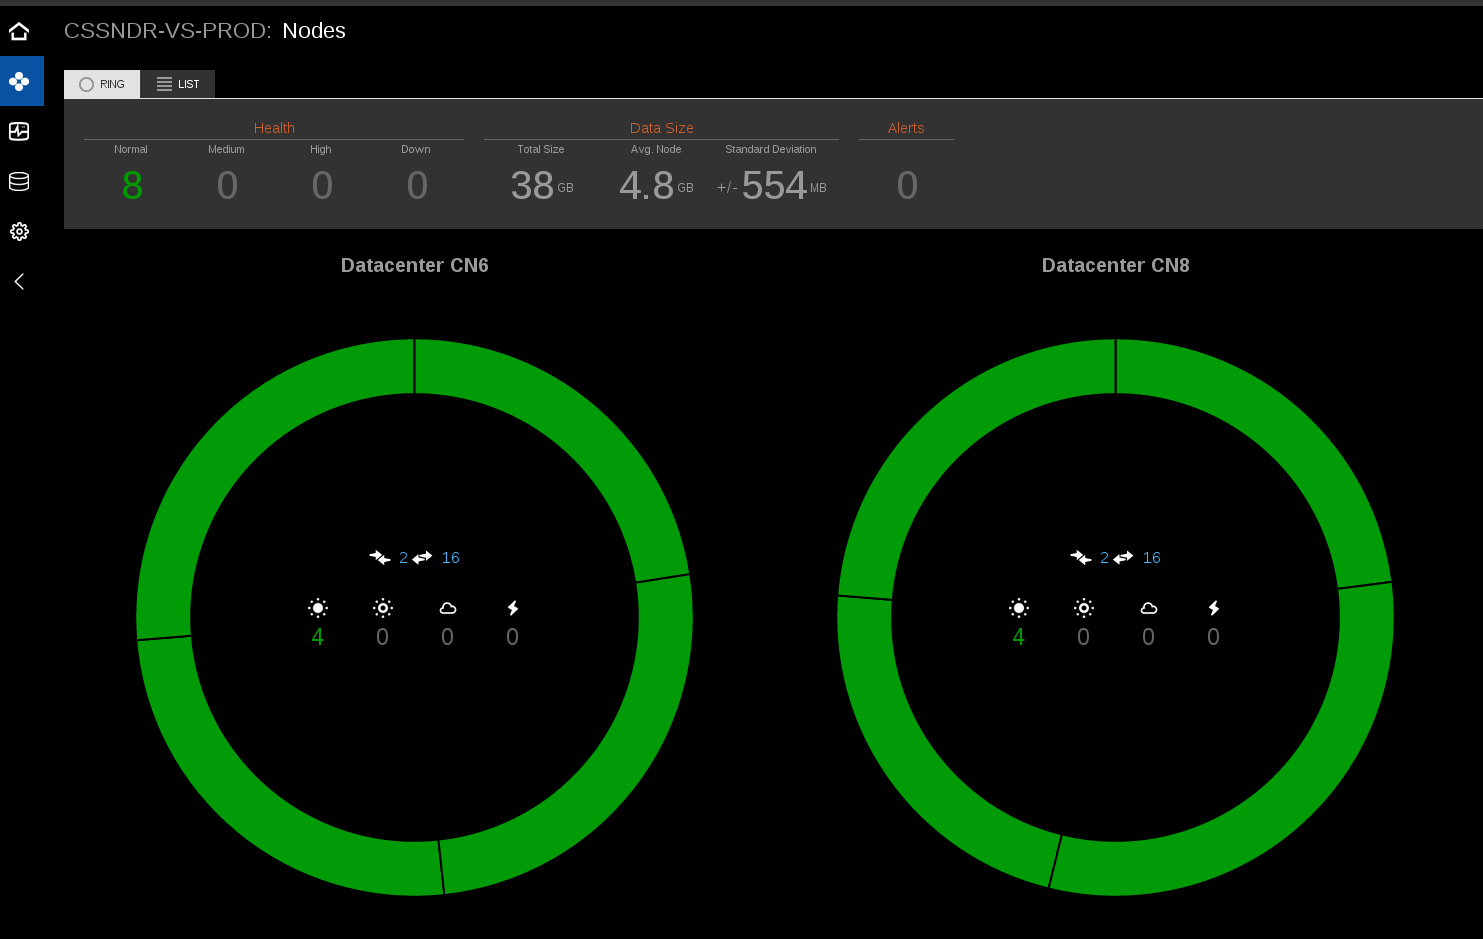
\includegraphics[scale=0.2]{./images/deployment-status}
    \end{center}
  \end{block}
\end{frame}

\begin{frame}{实时性能状态}
  \begin{center}
    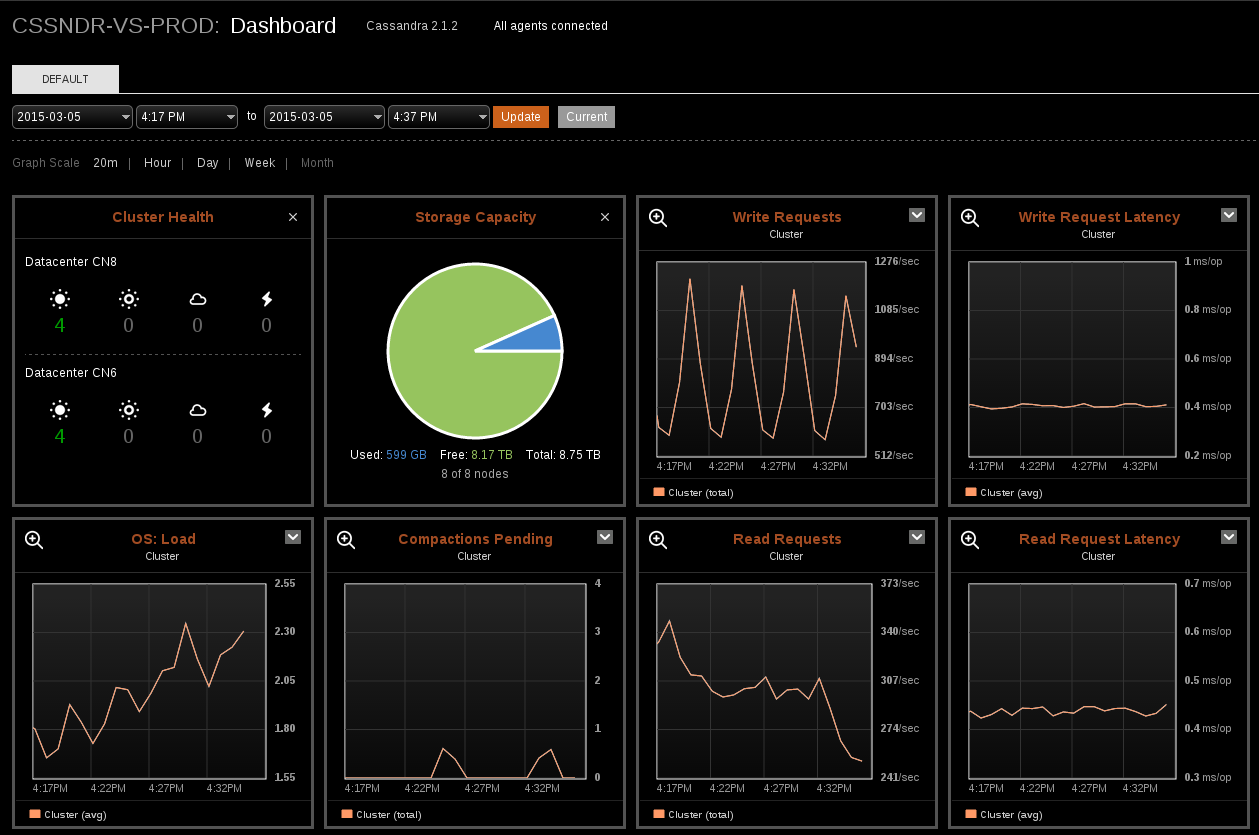
\includegraphics[scale=0.2]{./images/runtime-status}
  \end{center}
\end{frame}

\begin{frame}{在线应用}
  \begin{block}{页面静态元素}
    \begin{itemize}
      \item {访问量(pv)大}
      \item {一致性要求不高}
    \end{itemize}
  \end{block}
  \pause
  \begin{center}
    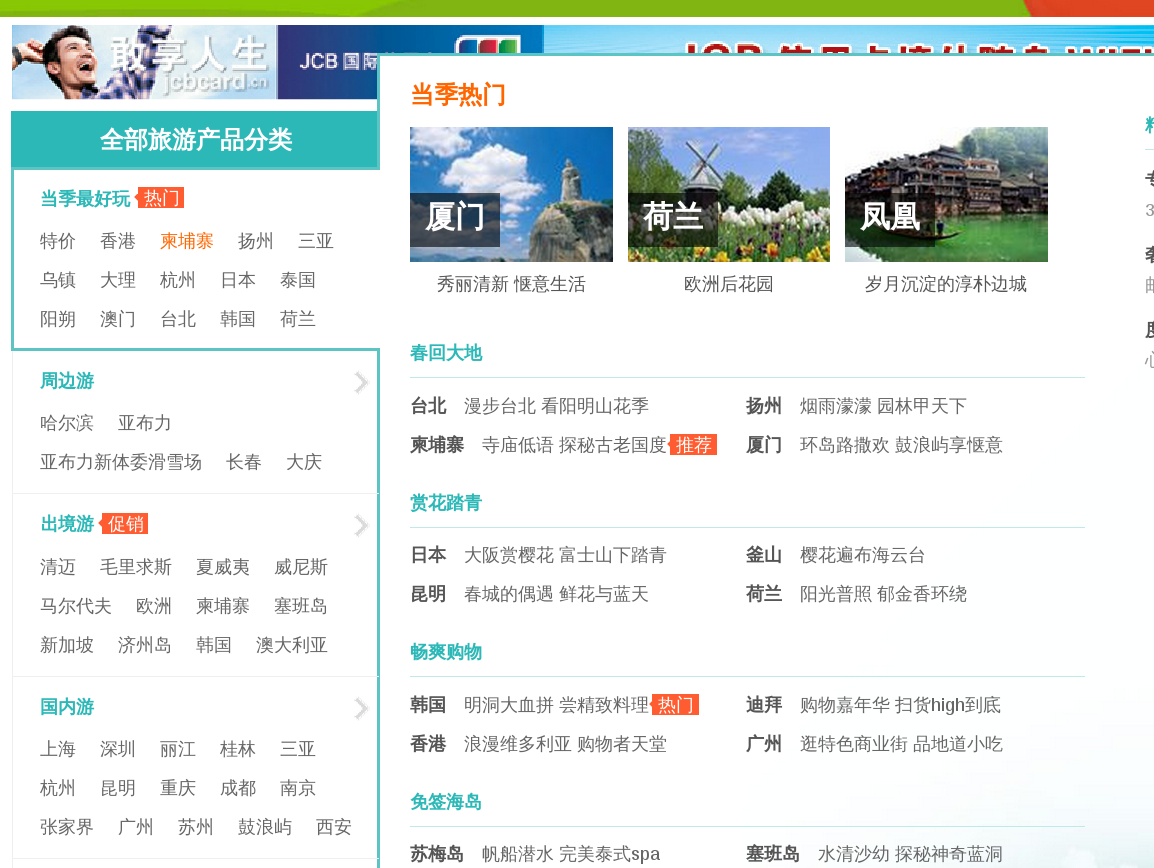
\includegraphics[scale=0.2]{./images/homepage-leftnav}
  \end{center}
\end{frame}

\begin{frame}{}
  \begin{block}{与业务逻辑相关的实时数据统计}
    \begin{itemize}
      \item {读取与写入都比较频繁}
      \item {一致性要求不高}
    \end{itemize}
  \end{block}
  \pause
  \begin{block}{应用举例}
    \begin{itemize}
      \item {用户进行搜索时,若长线游数量小于20,补充周边出发城市线路}
      \item {对每个用户搜索query进行实时搜索量监控}
    \end{itemize}
  \end{block}
\end{frame}

\begin{frame}{离线应用}
  \begin{block}{数据统计分析}
    \begin{itemize}
      \item {处理数据量和生成的数据量都比较大}
    \end{itemize}
  \end{block}
  \pause
  \begin{block}{应用举例}
    \begin{center}
      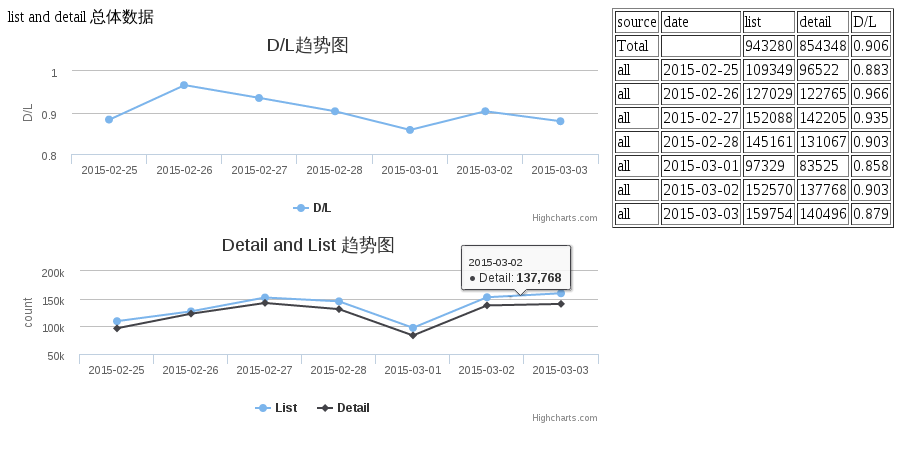
\includegraphics[scale=0.2]{./images/search-dashboard}
    \end{center}
  \end{block}
\end{frame}


% \subsection{Second Subsection}

% You can reveal the parts of a slide one at a time
% with the \pause command:
%% \begin{frame}{Second Slide Title}
%%   \begin{itemize}
%%   \item {
%%     First item.
%%     \pause % The slide will pause after showing the first item
%%   }
%%   \item {   
%%     Second item.
%%   }
%%   % You can also specify when the content should appear
%%   % by using <n->:
%%   \item<3-> {
%%     Third item.
%%   }
%%   \item<4-> {
%%     Fourth item.
%%   }
%%   % or you can use the \uncover command to reveal general
%%   % content (not just \items):
%%   \item<5-> {
%%     Fifth item. \uncover<6->{Extra text in the fifth item.}
%%   }
%%   \end{itemize}
%% \end{frame}


% Placing a * after \section means it will not show in the
% outline or table of contents.
\section*{总结}

\begin{frame}{总结}
  \begin{block}{Cassandra的主要特性}
    \begin{itemize}
      \item {无单点瓶颈}
      \item {可扩展性良好}
      \item {高性能并发读写}
      \item {根据业务需要调整数据一致性级别}
    \end{itemize}    
  \end{block}
  \begin{block}{技术实现原理}
  \begin{itemize}
    \item {一致性哈希}
    \item {Memtable, SSTable数据结构}
  \end{itemize}
  \end{block}
\end{frame}

\appendix
\section<presentation>*{\appendixname}
\subsection<presentation>*{参考资料}

\begin{frame}
  \frametitle<presentation>{参考资料}
    
  \begin{thebibliography}{10}
    
  \beamertemplatearticlebibitems
  % Followed by interesting articles. Keep the list short. 

  \bibitem{dynamo}
    Giuseppe DeCandia, et. al.
    \newblock {Dynamo: Amazon’s Highly Available Key-value Store}
    \newblock {\url{http://s3.amazonaws.com/AllThingsDistributed/sosp/amazon-dynamo-sosp2007.pdf}}

  \bibitem{bigtable}
    Chang, F., Dean, et. al.
    \newblock {Bigtable: A Distributed Storage System For Structured Data}
    \newblock {\url{http://research.google.com/archive/bigtable-osdi06.pdf}}

  \bibitem{introcssndr}
    Gary Dusbabek
    \newblock {Introduction to Cassandra}

  \end{thebibliography}

  \beamertemplate
\end{frame}


% All of the following is optional and typically not needed. 
%% \appendix
%% \section<presentation>*{\appendixname}
%% \subsection<presentation>*{For Further Reading}

%% \begin{frame}[allowframebreaks]
%%   \frametitle<presentation>{For Further Reading}
    
%%   \begin{thebibliography}{10}
    
%%   \beamertemplatebookbibitems
%%   % Start with overview books.

%%   \bibitem{Author1990}
%%     A.~Author.
%%     \newblock {\em Handbook of Everything}.
%%     \newblock Some Press, 1990.
 
    
%%   \beamertemplatearticlebibitems
%%   % Followed by interesting articles. Keep the list short. 

%%   \bibitem{Someone2000}
%%     S.~Someone.
%%     \newblock On this and that.
%%     \newblock {\em Journal of This and That}, 2(1):50--100,
%%     2000.
%%   \end{thebibliography}
%% \end{frame}

\clearpage
\end{CJK}
\end{document}
